% Drawing 142/06-7 -- folder 142, batch 06, archive page 107 (PDF page 108).
% Transcription: La seconde sphère : petit cercle orienté autour du pôle supérieur et autour de $\infty$ en bas ; sur l'équateur, cercles autour de $1$ et $-1$, points $-i$ et $i$ ; chemins marqués $\beta$, « $\beta$ relevé », « $\gamma$ relevé » (deux fois), le dernier avec la mention « $\gamma$ relevé, symétrique de \ill{} ».
% Kind: sphere with pole circles, equatorial circles and lifted paths. Method 2 (schematic redraw from the facsimile). Status: partial.
% Notes: In pencil and ink: outline, a small oriented circle round the upper pole and one round infinity at the bottom; the dashed equator with the circles round 1 (left) and -1 (right) and the points -i, i; the meridians and the paths marked beta (with a tilde above, a bar on the right), "beta releve" (twice), "gamma releve" and "gamma releve, symetrique de ..." (the last word illegible, left out). The label at the upper pole reads like infinity as well; it is left unlabelled, as in the transcription. The formula on the right (l_infty l_1 l_0 ...) is text, not drawn.
% Coordinates: 1 unit = 1 mm = 1/100 of the crop width (bbox in page fractions: [0.1, 0.43, 0.68, 0.72]).
% Redrawn by Claude (claude-opus-5-5), issue #73, 2026-11-07; not checked by a human; not compiled (no TeX in the session).
% Rights: reproduces part of the work -- behind RENDER_TRANSCRIPTS, never published by itself.
\documentclass[tikz,border=3pt]{standalone}
\usepackage{amsmath,amssymb}
\usetikzlibrary{patterns,arrows.meta}
\tikzset{pencil/.style={black!45}, struck/.style={black!35}, mark/.style={circle,draw,inner sep=1.3pt}, pt/.style={circle,fill,inner sep=0.9pt}, opt/.style={circle,draw,fill=white,inner sep=1.1pt}}
\begin{document}
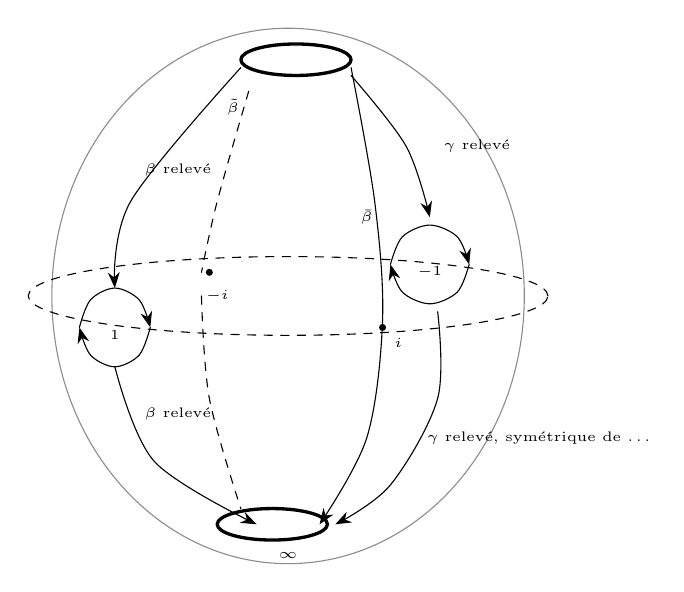
\begin{tikzpicture}[x=1mm,y=1mm,line cap=round,line join=round,font=\scriptsize]
\draw[pencil] (42,-37) ellipse[x radius=30, y radius=34];
\draw[very thick] (43,-7) ellipse[x radius=7, y radius=2];
\draw[very thick] (40,-66) ellipse[x radius=7, y radius=2];
\node[inner sep=1pt] at (42,-70) {\tiny $\infty$};
\draw[dashed] (42,-37) ellipse[x radius=33, y radius=5];
\draw[-{Stealth[length=2mm]}] plot[smooth, tension=0.55] coordinates {(15.5,-41) (16.9,-37.5) (20,-36) (23.1,-37.5) (24.5,-41)};
\draw[-{Stealth[length=2mm]}] plot[smooth, tension=0.55] coordinates {(24.5,-41) (23.1,-44.5) (20,-46) (16.9,-44.5) (15.5,-41)};
\draw[-{Stealth[length=2mm]}] plot[smooth, tension=0.55] coordinates {(55,-33) (56.5,-29.5) (60,-28) (63.5,-29.5) (65,-33)};
\draw[-{Stealth[length=2mm]}] plot[smooth, tension=0.55] coordinates {(65,-33) (63.5,-36.5) (60,-38) (56.5,-36.5) (55,-33)};
\node[inner sep=1pt] at (20,-42) {\tiny $1$};
\node[inner sep=1pt] at (60,-34) {\tiny $-1$};
\node[pt] at (32,-34) {};
\node[pt] at (54,-41) {};
\node[inner sep=1pt] at (33,-37) {\tiny $-i$};
\node[inner sep=1pt] at (56,-43) {\tiny $i$};
\draw[-{Stealth[length=2mm]}] plot[smooth, tension=0.55] coordinates {(36,-8) (22,-25) (20,-36)};
\draw[-{Stealth[length=2mm]}] plot[smooth, tension=0.55] coordinates {(20,-46) (25,-58) (38,-66)};
\draw[-{Stealth[length=2mm]}] plot[smooth, tension=0.55] coordinates {(50,-8) (53,-25) (54,-40) (52,-55) (46,-66)};
\draw[dashed] plot[smooth, tension=0.55] coordinates {(37,-11) (33,-25) (31,-34)};
\draw[dashed] plot[smooth, tension=0.55] coordinates {(31,-37) (32,-50) (36,-64)};
\draw[-{Stealth[length=2mm]}] plot[smooth, tension=0.55] coordinates {(50,-9) (57,-18) (60,-27)};
\draw[-{Stealth[length=2mm]}] plot[smooth, tension=0.55] coordinates {(61,-39) (61,-50) (55,-61) (48,-66)};
\node[inner sep=1pt] at (35,-13) {\tiny $\tilde\beta$};
\node[inner sep=1pt] at (28,-21) {\tiny $\beta$ relev\'e};
\node[inner sep=1pt] at (52,-27) {\tiny $\bar\beta$};
\node[inner sep=1pt] at (66,-18) {\tiny $\gamma$ relev\'e};
\node[inner sep=1pt] at (28,-52) {\tiny $\beta$ relev\'e};
\node[inner sep=1pt] at (74,-55) {\tiny $\gamma$ relev\'e, sym\'etrique de \dots};
\end{tikzpicture}
\end{document}
